\newcommand{\defaultparindent}{\parindent}
\setlength{\parindent}{0pt}				% \noindent partout
% \parindent in one-column documents is :
% 15pt when the default text size is 10pt,
% 17pt for 11pt,
% and 1.5em for 12pt.
% In two-column documents it is 1em

%\begin{center}
%\begin{tabular}{p{5cm} p{11cm}}
%\textbf{Commandes étudiées :} & \texttt{sh}, \texttt{bash}, \texttt{man}, \texttt{ls}, \texttt{mkdir}, \texttt{touch}, \texttt{chmod}, \texttt{mv}, \texttt{rm}, \texttt{rmdir}, \texttt{cat}, \texttt{file}, \texttt{whereis}, \texttt{which}\\

%\textbf{Builtins étudiées :} & \texttt{pwd}, \texttt{cd}, \texttt{exit}, \texttt{logout}, \texttt{echo}, \texttt{umask}, \texttt{type}, \texttt{>}, \texttt{>{}>}, \texttt{<}, \texttt{<{}<}, \texttt{|}\\

%\textbf{Notions étudiées :} & Tableaux, Pointeurs, Files\\
%\end{tabular}
%\end{center}

\textbf{Notions étudiées :} Tableaux, Pointeurs, Files\\

%\bigskip

\subsection{Rappel sur les piles}

\bigskip

Les \textbf{piles}, ou \textbf{stacks} en anglais, sont des structures visant à stocker les données dans l'ordre d'arrivée, mais ne permettant leur récupération uniquement dans l'ordre inverse.
Dans une pile, on ne peut accéder qu'à la dernière donnée stockée, celle se situant au \textit{sommet} de la pile.
Ces structures sont aussi appelées \textbf{LIFO} (\textit{Last In First Out}).\\

\begin{center}
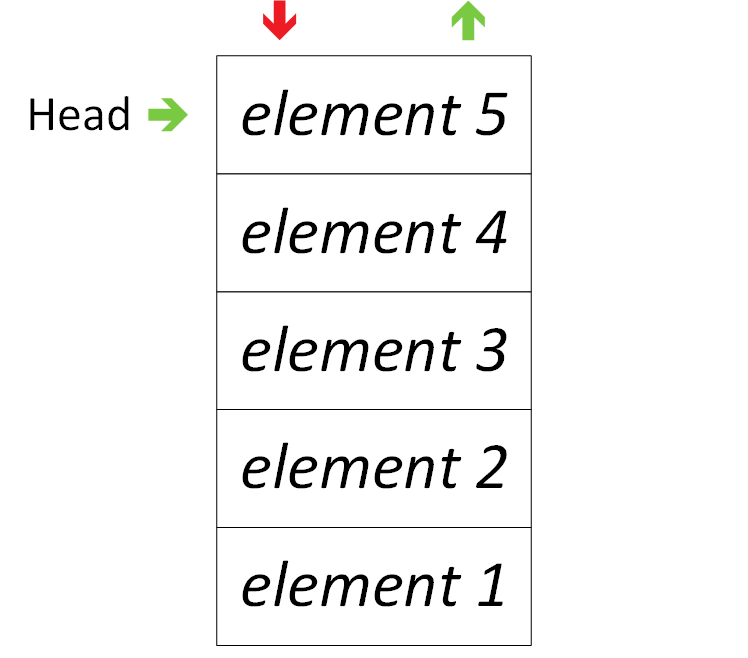
\includegraphics[scale=0.75]{Cours/Piles_1_Structure_Generale_centered.png}
\end{center}

\smallskip

Deux opérations permettent d'utiliser une pile :
\begin{itemize}
\item \TTBF{PUSH} : permettant d'\textit{empiler} une donnée supplémentaire dans la pile
\item \TTBF{POP} : permettant de \textit{dépiler} une donnée depuis la pile
\end{itemize}
On ajoute donc une donnée en l'empilant avec un \TTBF{PUSH}, et il est possible de directement y accéder, car elle est au sommet de la pile.
À l'inverse, pour accéder à une donnée tout au fond de la pile, il est nécessaire de dépiler autant d'éléments que nécessaire avec un \TTBF{POP}.\\

Voici un exemple où l'on crée une pile, puis on empile successivement $ 42 $, $ 5 $, et $ 13 $, puis, on dépile une fois (pour récupérer $ 13 $), et enfin, on empile successivement $ 37 $, $ 10 $, $ 24 $.\\

\begin{center}
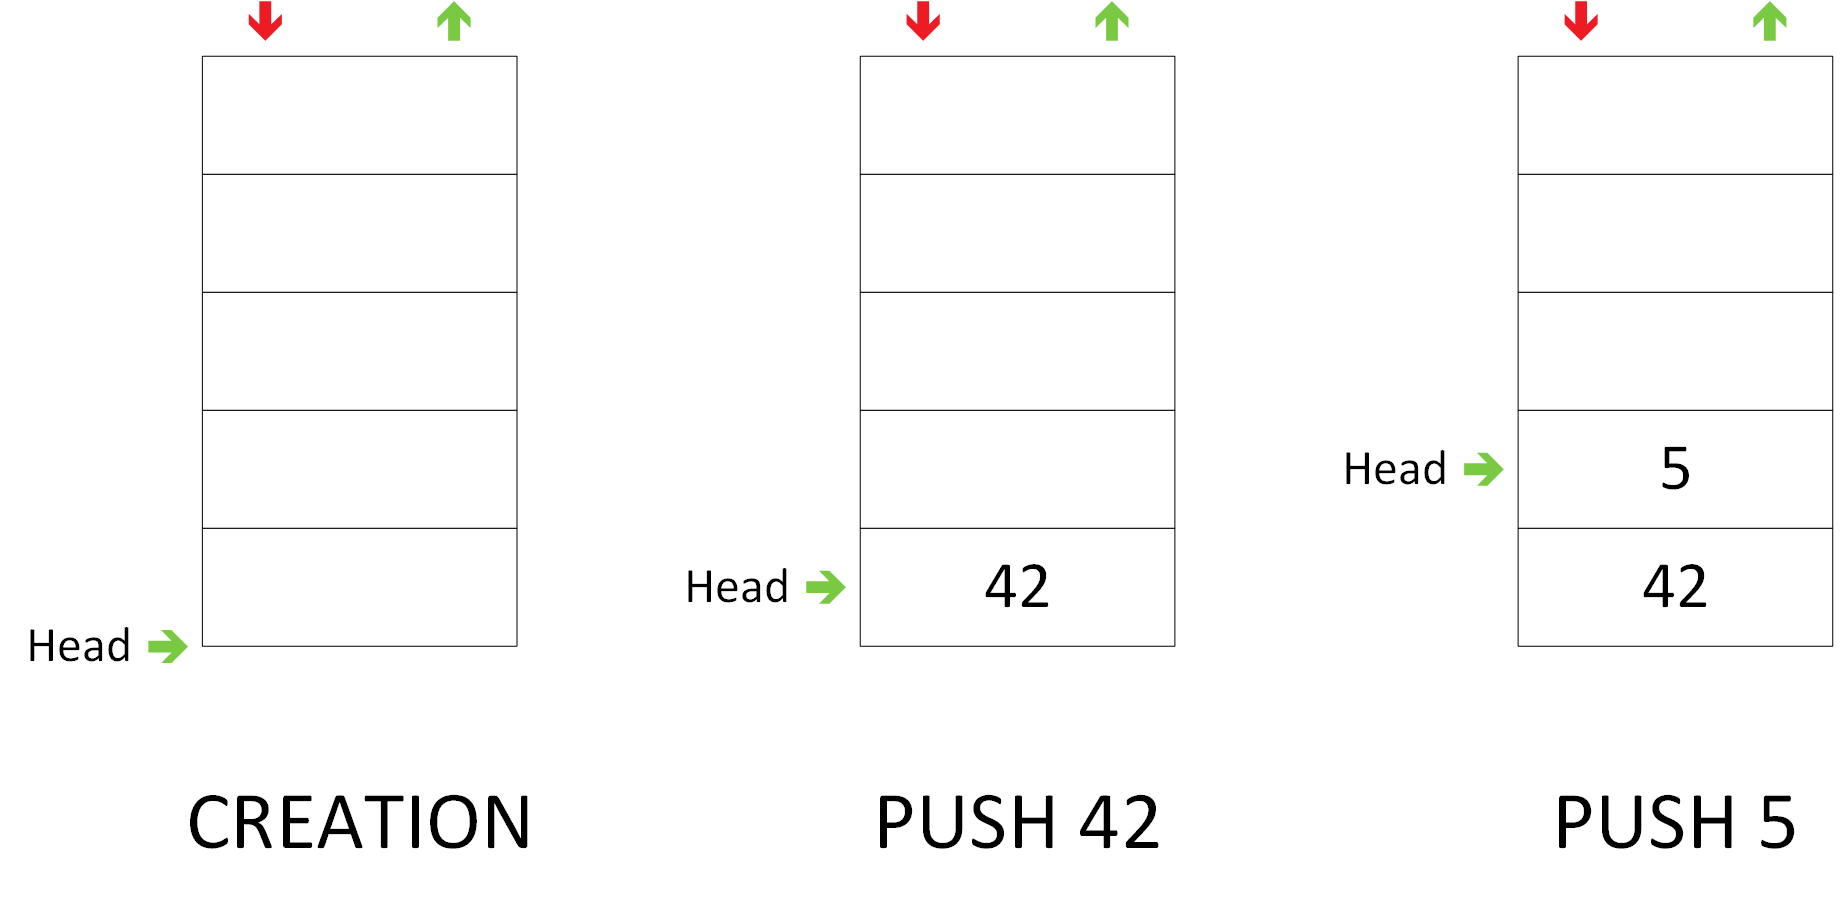
\includegraphics[scale=0.5]{Cours/Piles_2_Structure_Generale_Usage_pack_1.png}
\end{center}

\begin{center}
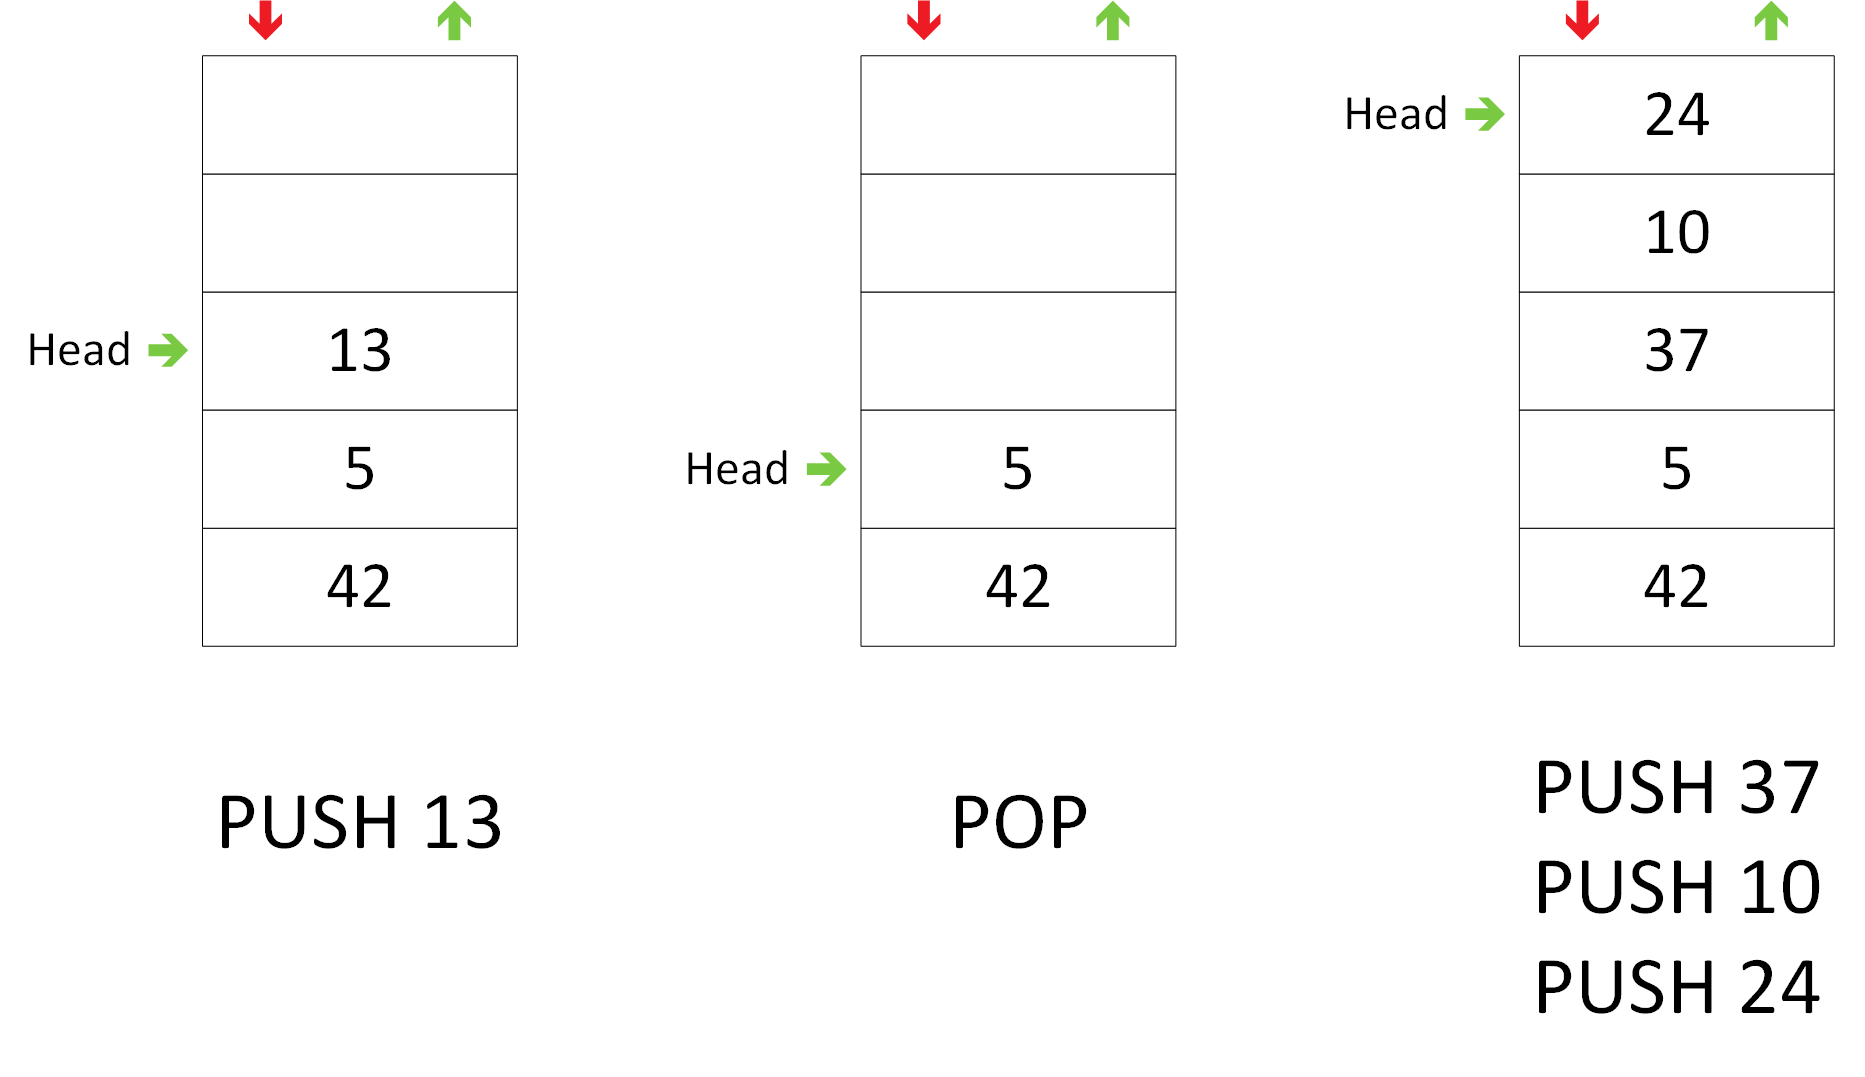
\includegraphics[scale=0.5]{Cours/Piles_2_Structure_Generale_Usage_pack_2.png}
\end{center}

\smallskip

Les piles, et surtout la contrainte d'accès aux objets, sont couramment utilisées : un camion de livraison sera d'abord rempli avec les paquets à livrer en dernier/le camion sera rempli dans l'ordre inverse de livraison (on accède d'abord aux derniers éléments chargés).

En informatique, on utilisera les piles dans certains \textit{parsers} (analyse grammaticale) pour connaître en premier l'opérateur à exécuter (opérateur binaire ? unaire ?) et dépiler par la suite le nombre exact de paramètres.
La \textit{pile d'appels} est également une convention fondamentale partagée par les processeurs et les systèmes d'exploitation permettant de passer des paramètres (et d'autres informations de contexte) aux fonctions appelées par les programmes, ou en cas d'interruption pour sauvegarder l'adresse de l'instruction qui était en cours d'exécution.\\

Afin d'implémenter une pile, il est donc nécessaire d'avoir un espace de stockage ordonné (un tableau numéroté ou une liste chaînée), et un indicateur de l'élément en haut de la pile.
Nous allons maintenant voir comment implémenter une pile avec des listes chaînées et un tableau de taille fixe.

\bigskip

%%%%%%%%%%%%%%%%%%%%%%%%%%%%%%%%%%%%%%%%%%%%%%%%%%%%%%%%%%%%
%%%%%%%%%%%%%%%%%%%%%%%%%%%%%%%%%%%%%%%%%%%%%%%%%%%%%%%%%%%%
%%%%%%%%%%%%%%%%%%%%%%%%%%%%%%%%%%%%%%%%%%%%%%%%%%%%%%%%%%%%

\subsection{Piles : implémentation avec des listes chaînées}

\bigskip

Une implémentation à l'aide d'une liste chaînée permet d'exploiter la mémoire et d'être donc beaucoup plus flexible en terme de nombre maximum d'éléments.
Le schéma suivant illustre une pile sous forme de liste chaînée en mémoire :\\

\begin{center}
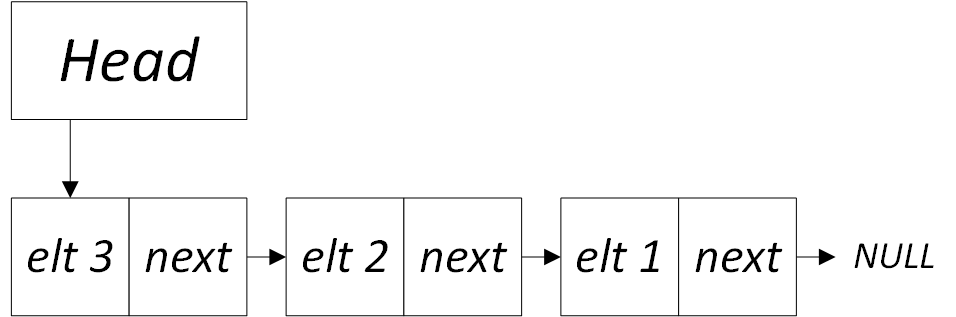
\includegraphics[scale=0.75]{Cours/Piles_3_Liste_Chainee_Structure_cas_general.png}
\end{center}

\smallskip

On y retrouve plusieurs fois la structure typique des listes chaînées (un élément et un pointeur vers l'élément suivant), ainsi qu'un pointeur indiquant le sommet de la pile (\textit{head} dans notre cas).

L'unique cas particulier concerne une pile vide : le pointeur de sommet vaut dans ce cas \TTBF{NULL}.
Il s'agit également de l'état dans lequel se trouve une pile vidée ou nouvellement créée.\\

\begin{center}
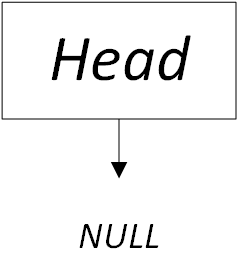
\includegraphics[scale=0.75]{Cours/Piles_3_Liste_Chainee_Structure_cas_vide.png}
\end{center}

\smallskip

L'exemple suivant montre l'évolution d'une pile au fur et à mesure des ajouts (empiler / \TTBF{PUSH}) et suppressions (dépiler / \TTBF{POP}).\\

\begin{center}
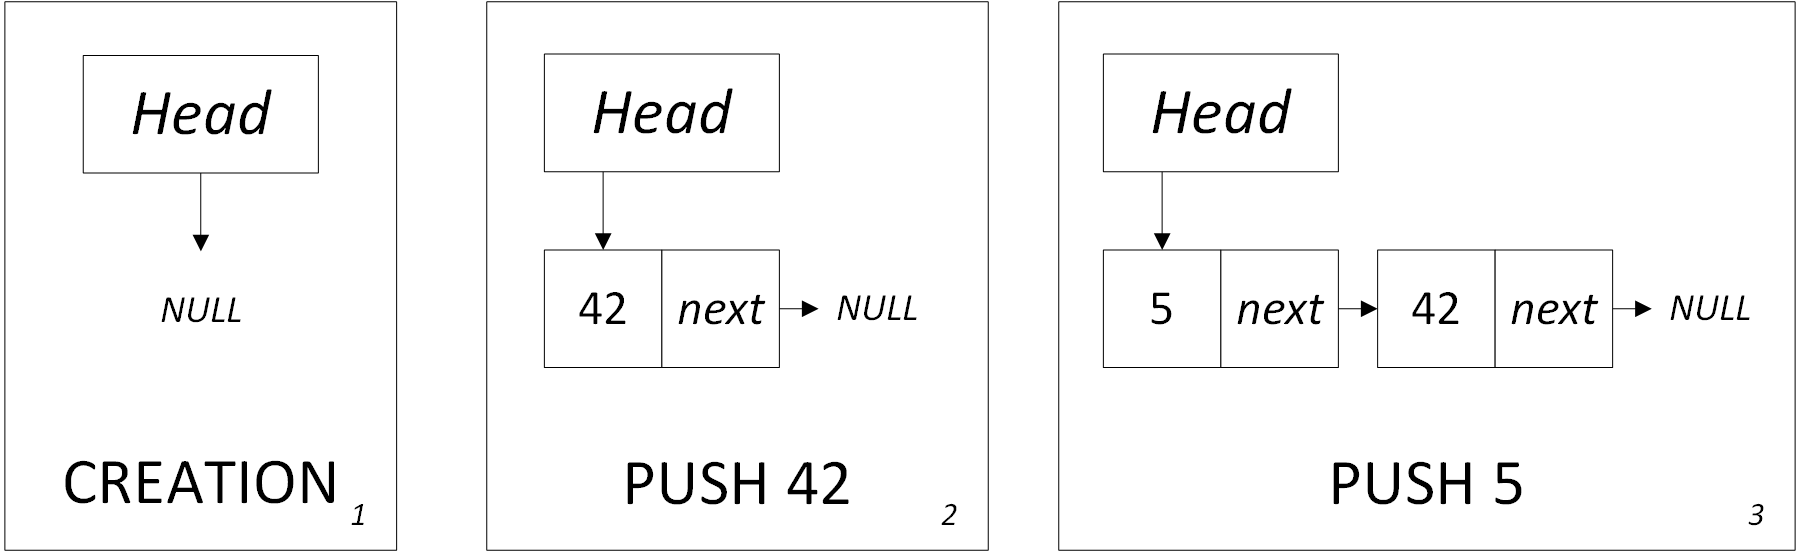
\includegraphics[scale=0.65]{Cours/Piles_4_Liste_Chainee_Usage_pack_1.png}
\end{center}

\begin{center}
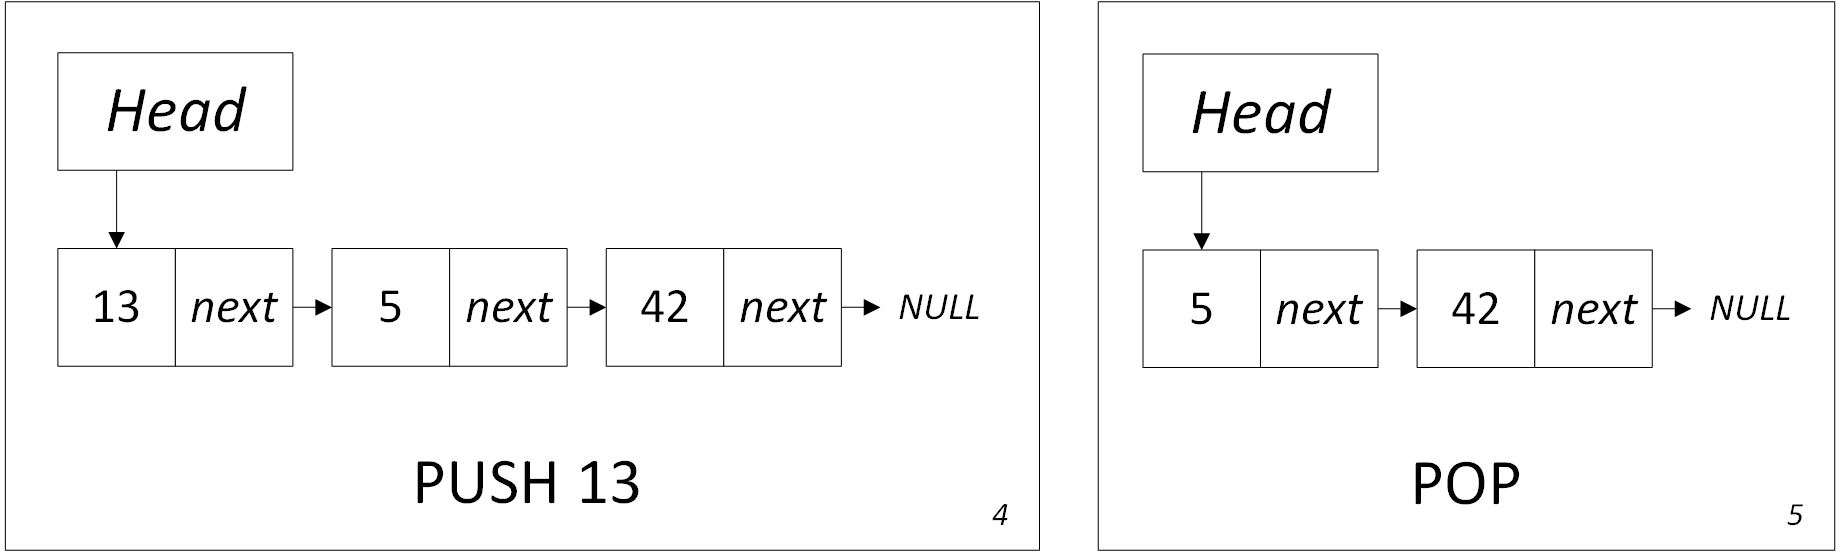
\includegraphics[scale=0.65]{Cours/Piles_4_Liste_Chainee_Usage_pack_2.png}
\end{center}

\smallskip

Les principales opérations se résument ainsi :
\begin{itemize}
\item Création : on alloue en mémoire la structure générale de la pile, et on fixe le sommet de la pile à \TTBF{NULL}.
\item Empiler : on alloue en mémoire un nouvel élément dont le pointeur \textit{next} pointe vers l'actuel élément au sommet de la pile, puis, on met à jour le pointeur de sommet de la pile vers l'adresse de ce nouvel élément.
\item Dépiler : si la pile est vide, on retourne une erreur, sinon, on récupère tout d'abord l'adresse de l'élément suivant celui au sommet, puis, on libère l'élément au sommet, puis, on met à jour le pointeur de sommet de la pile vers l'adresse de l'élément suivant.
\item Vider : on dépile successivement tous les éléments jusqu'à obtenir un sommet à \TTBF{NULL}.
\item Sommet : on renvoie le contenu de l'élément au sommet de la pile.
\end{itemize}

\bigskip

%%%%%%%%%%%%%%%%%%%%%%%%%%%%%%%%%%%%%%%%%%%%%%%%%%%%%%%%%%%%
%%%%%%%%%%%%%%%%%%%%%%%%%%%%%%%%%%%%%%%%%%%%%%%%%%%%%%%%%%%%
%%%%%%%%%%%%%%%%%%%%%%%%%%%%%%%%%%%%%%%%%%%%%%%%%%%%%%%%%%%%

\subsection{Rappel sur les files}

\bigskip

Les \textbf{files}, ou \textbf{queues} en anglais, sont des structures visant à stocker et rendre les données dans l'ordre d'arrivée.
Une file dispose donc d'une \textit{tête} contenant l'élément le plus ancien (inséré avant tous les autres), et une \textit{queue} contenant l'élément inséré le plus récemment.
Ces structures sont aussi appelées \textbf{FIFO} (\textit{First In First Out}).\\

\begin{center}
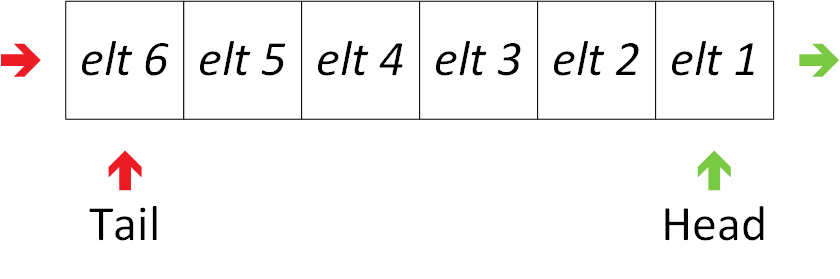
\includegraphics[scale=0.75]{Cours/Files_1_Structure_Generale.png}
\end{center}

\smallskip

Deux opérations permettent d'utiliser une file :
\begin{itemize}
\item \TTBF{ENQUEUE} : permettant d'\textit{enfiler} une donnée supplémentaire dans la file
\item \TTBF{DEQUEUE} : permettant de \textit{défiler} une donnée depuis la file
\end{itemize}
On ajoute donc une donnée en l'enfilant avec un \TTBF{ENQUEUE}, celle-ci se retrouve en \textit{queue} de file, c'est-à-dire au fond de la file.
On récupère une donnée en défilant avec un \TTBF{DEQUEUE}, celle-ci se trouvait en \textit{tête} de file, c'est-à-dire qu'elle attendait son tour depuis son insertion.
On accède donc aux éléments dans l'ordre d'arrivée.\\

Voici un exemple où l'on crée une file, puis on enfile successivement $ 42 $, $ 5 $, et $ 13 $, puis, on défile une fois (pour récupérer $ 42 $), et enfin, on enfile successivement $ 37 $, $ 10 $, $ 24 $, et $ 8 $.\\

\begin{center}
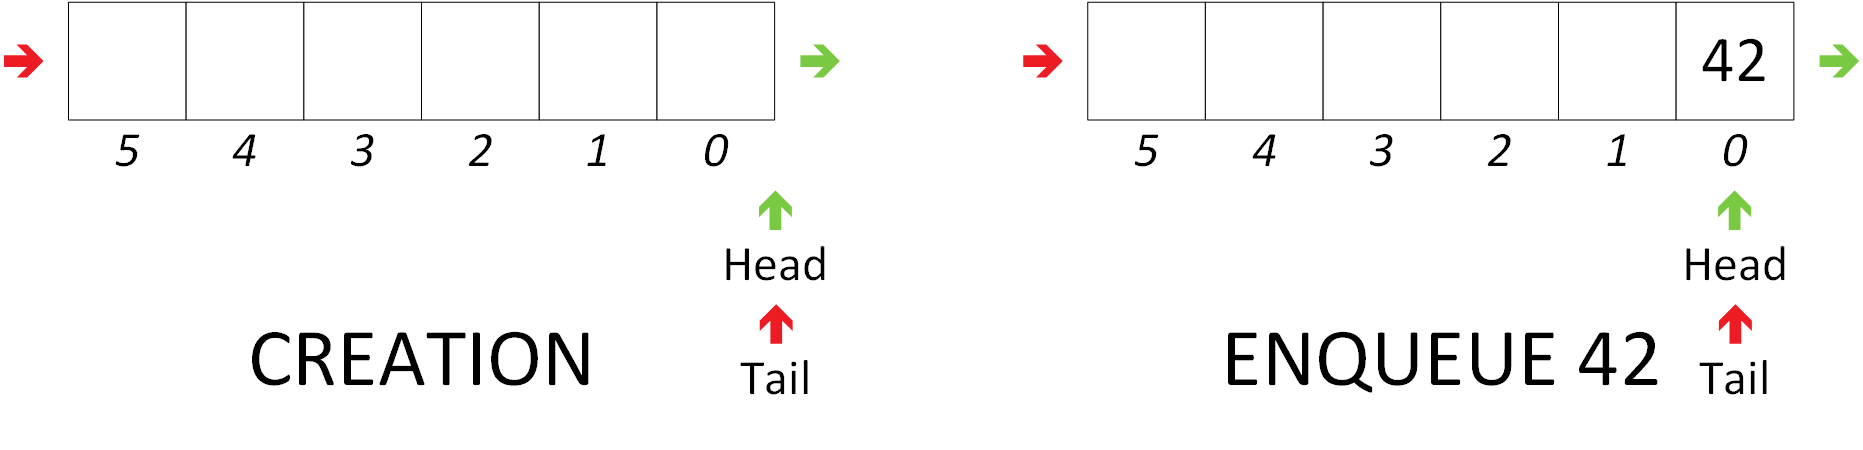
\includegraphics[scale=0.65]{Cours/Files_2_Structure_Generale_Usage_pack_1.png}
\end{center}

\begin{center}
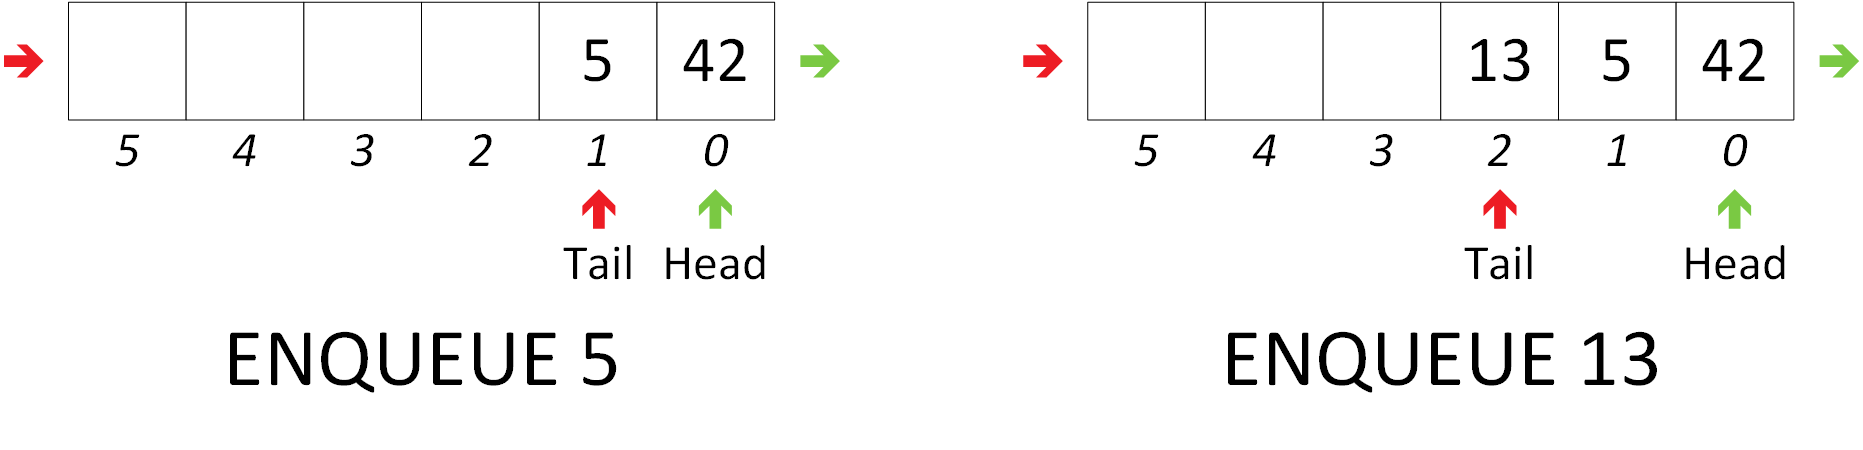
\includegraphics[scale=0.65]{Cours/Files_2_Structure_Generale_Usage_pack_2.png}
\end{center}

\begin{center}
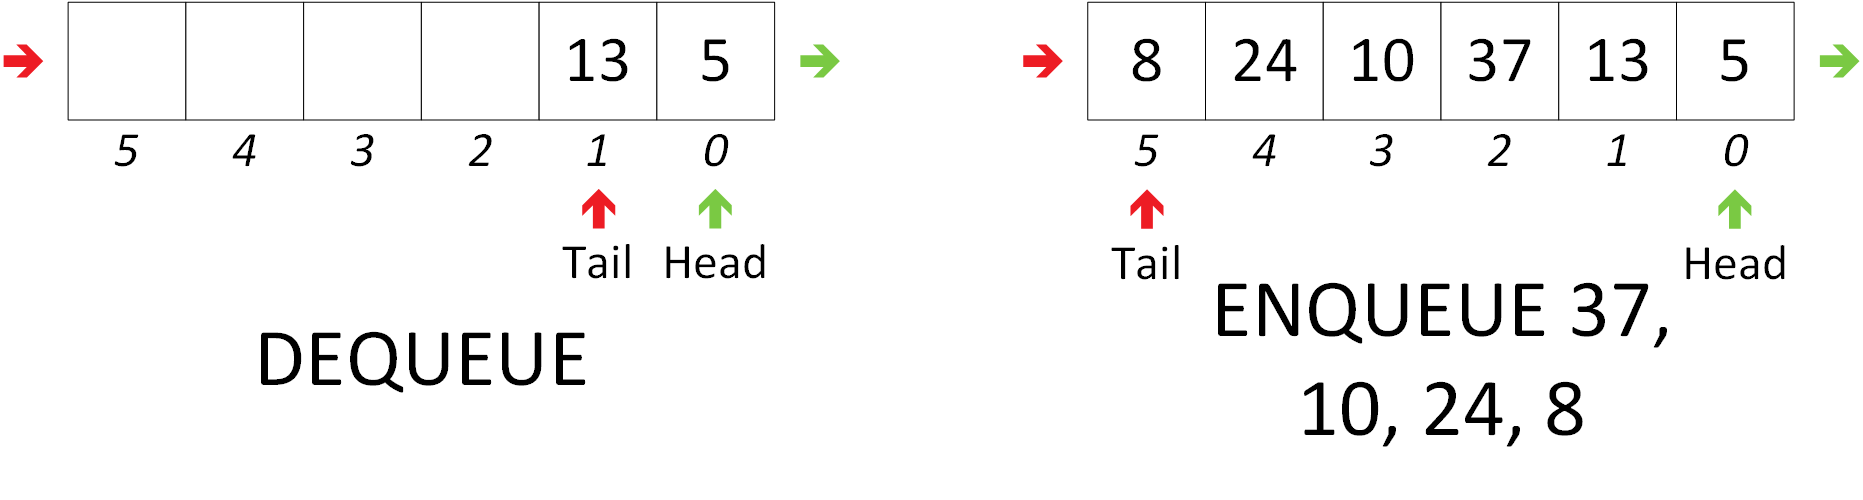
\includegraphics[scale=0.65]{Cours/Files_2_Structure_Generale_Usage_pack_3.png}
\end{center}

\smallskip

Les files, et surtout le respect de l'ordre d'arrivée des objets, sont couramment utilisés : mise en attente de personnes face à des guichets (voitures à un péage, clients face à une caisse, etc).

En informatique, on utilisera les files pour stocker temporairement et traiter les requêtes dans leur ordre d'arrivée.
Dans le cas des \textit{schedulers} (ordonnanceurs) visant à déterminer quel processus exécuter sur le c\oe{}ur d'un processus, on ajoute parfois une priorité à chaque objet de la file.
Ceci implique de mettre à jour l'ordre des objets dans la file lors de certains évènements (par exemple lorsque l'on enfile ou défile un élément, ou après un certain temps).\\

Afin d'implémenter une file, il est donc nécessaire d'avoir un espace de stockage ordonné (un tableau numéroté ou une liste chaînée), et deux indicateurs pour l'élément tête de file et l'élément en queue de file.
Nous allons maintenant voir comment implémenter une file avec des listes chaînées et un tableau de taille fixe.

\bigskip

%%%%%%%%%%%%%%%%%%%%%%%%%%%%%%%%%%%%%%%%%%%%%%%%%%%%%%%%%%%%
%%%%%%%%%%%%%%%%%%%%%%%%%%%%%%%%%%%%%%%%%%%%%%%%%%%%%%%%%%%%
%%%%%%%%%%%%%%%%%%%%%%%%%%%%%%%%%%%%%%%%%%%%%%%%%%%%%%%%%%%%

\subsection{Files : implémentation avec des listes chaînées}

\bigskip

Une implémentation à l'aide d'une liste chaînée permet d'exploiter la mémoire et d'être donc beaucoup plus flexible en terme de nombre maximum d'éléments.
Le schéma suivant illustre une file sous forme de liste chaînée en mémoire :\\

\begin{center}
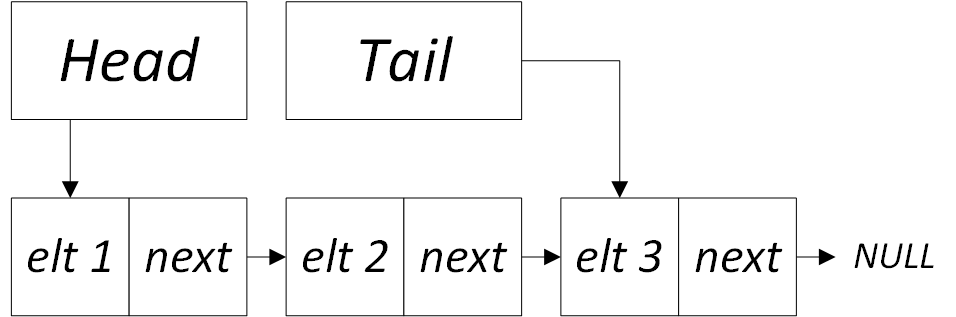
\includegraphics[scale=0.75]{Cours/Files_3_Liste_Chainee_Structure_cas_general.png}
\end{center}

\smallskip

On y retrouve plusieurs fois la structure typique des listes chaînées (un élément et un pointeur vers l'élément suivant), ainsi que deux pointeurs indiquant respectivement la tête de la file (\textit{head}) et la queue de la file (\textit{tail}).

Deux cas particuliers concernent les files où le pointeur de tête et le pointeur de queue valent la même chose : la file vide où les pointeurs contiennent \TTBF{NULL}, et la file contenant un seul élément vers lequel les deux pointeurs renvoient.
Une file nouvellement créée se trouve dans l'état vide.\\

\begin{center}
%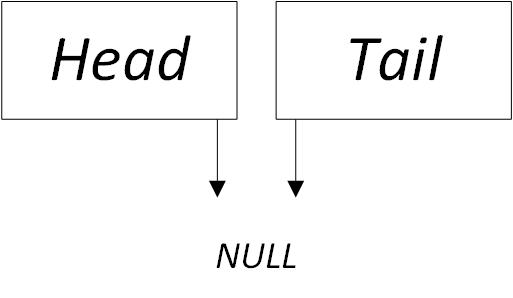
\includegraphics[scale=0.75]{Cours/Files_3_Liste_Chainee_Structure_cas_vide.png}
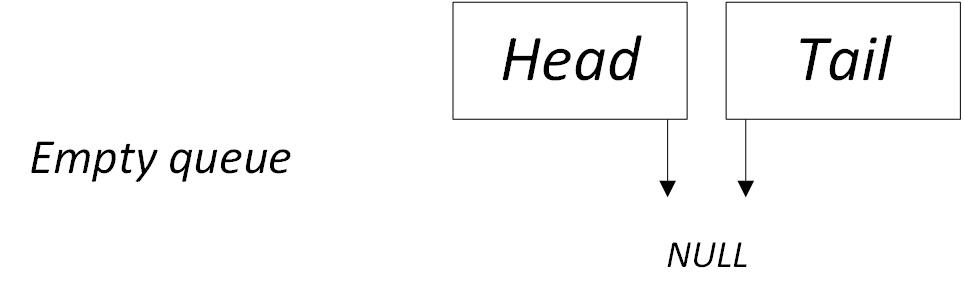
\includegraphics[scale=0.75]{Cours/Files_3_Liste_Chainee_Structure_cas_vide_etiquette.png}
\end{center}

\smallskip

\begin{center}
%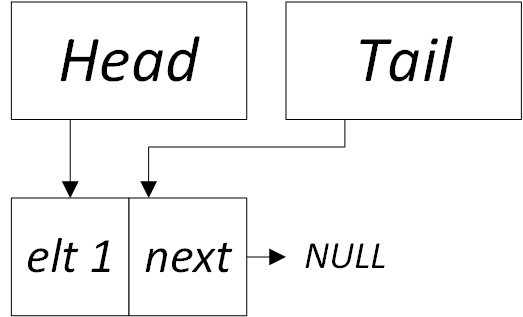
\includegraphics[scale=0.75]{Cours/Files_3_Liste_Chainee_Structure_cas_1_elt.png}
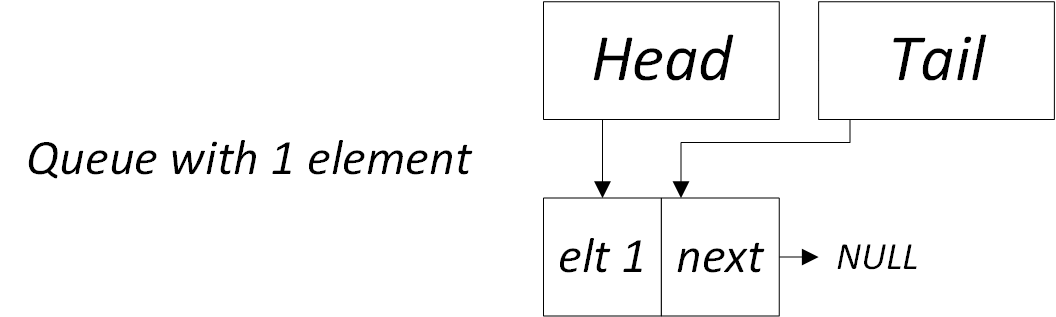
\includegraphics[scale=0.75]{Cours/Files_3_Liste_Chainee_Structure_cas_1_elt_etiquette.png}
\end{center}

\smallskip

L'exemple suivant montre l'évolution d'une file au fur et à mesure des insertions (enfiler / \TTBF{ENQUEUE}) et suppressions (défiler / \TTBF{DEQUEUE}).\\

\begin{center}
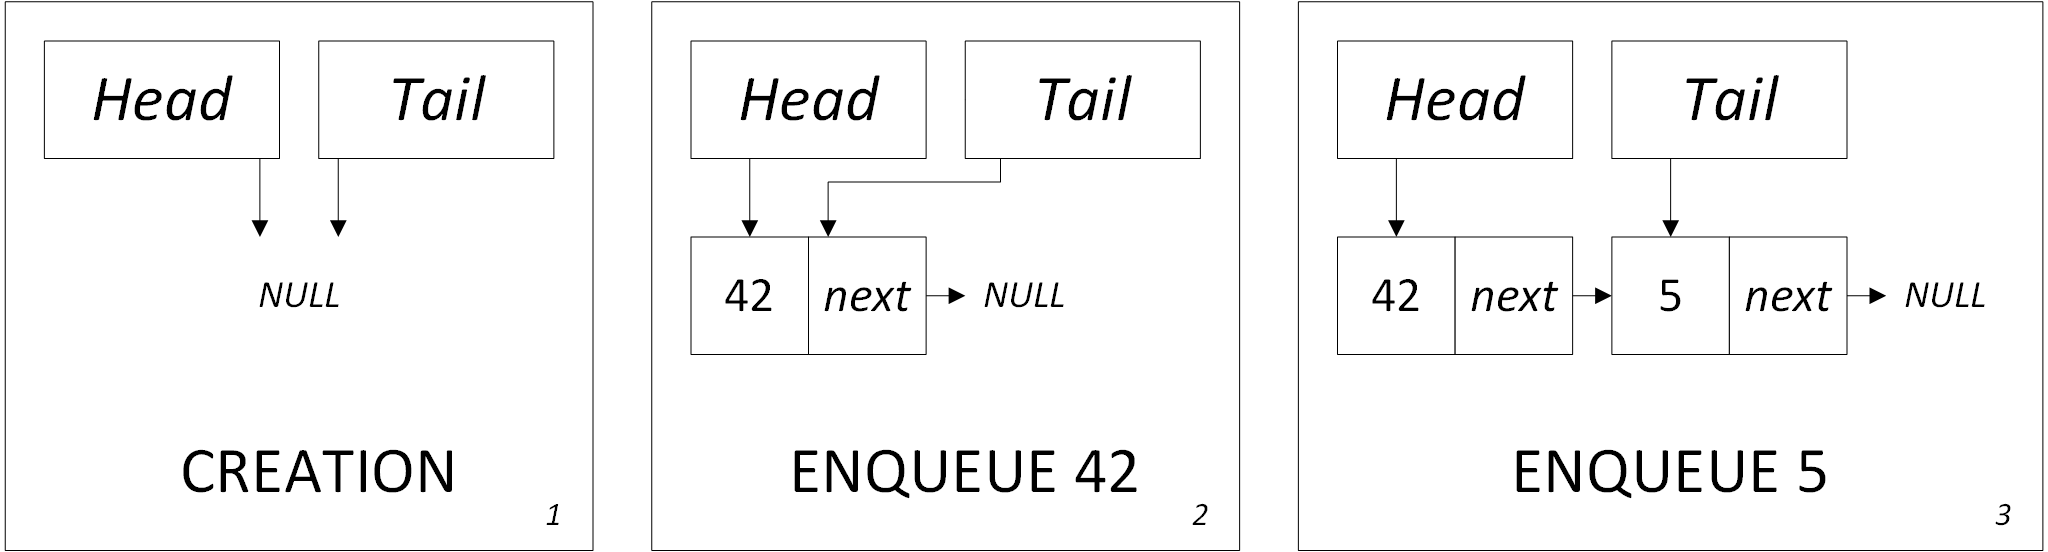
\includegraphics[scale=0.60]{Cours/Files_4_Liste_Chainee_Usage_pack_1.png}
\end{center}

\begin{center}
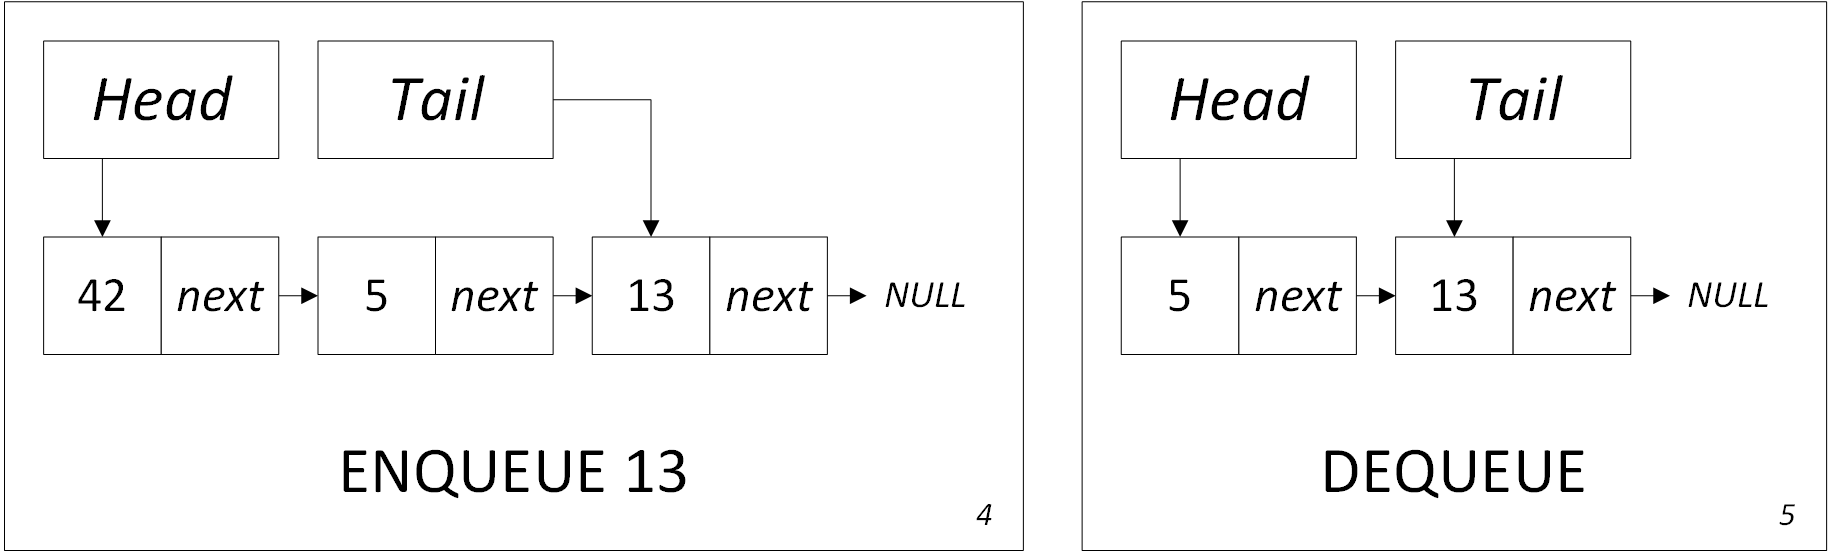
\includegraphics[scale=0.60]{Cours/Files_4_Liste_Chainee_Usage_pack_2.png}
\end{center}

\smallskip

Les principales opérations se résument ainsi :
\begin{itemize}
\item Création : on alloue en mémoire la structure générale de la file, et on fixe les tête et queue de la file à \TTBF{NULL}.
\item Enfiler : on alloue en mémoire un nouvel élément, on met son pointeur \textit{next} à \TTBF{NULL}, puis, si la file est vide, on met les pointeurs de tête et de queue sur le nouvel élément, sinon, on met l'adresse du nouvel élément sur le pointeur \textit{next} de l'élément pointé par la queue, et on met à jour le pointeur de queue sur le nouvel élément.
\item Défiler : si la file est vide, on retourne une erreur, sinon, on récupère tout d'abord l'adresse de l'élément suivant celui en tête, puis, on libère l'élément en tête, puis, on met à jour le pointeur de tête de la file vers l'adresse de l'élément suivant. Si l'élément suivant est \TTBF{NULL}, on met à jour le pointeur de queue également.
\item Vider : on défile successivement tous les éléments jusqu'à obtenir la tête à \TTBF{NULL} (ne pas oublier que l'opération qui défile met à jour la queue dans le cas \TTBF{NULL}).
\item Tête : on renvoie le contenu de l'élément en tête de file (le prochain élément qui sera défilé).
\item Queue : on renvoie le contenu de l'élément en queue de file (le dernier élément qui sera défilé).
\end{itemize}

\setlength{\parindent}{\defaultparindent}
